\documentclass[a4paper]{article}

\usepackage[francais,english]{babel}
\usepackage[T1]{fontenc}
\usepackage[]{fullpage}
\usepackage{graphicx}
\usepackage{hyperref}
\usepackage[utf8]{inputenc}
\usepackage{subfigure}

\makeatletter
\def\thickhrulefill{\leavevmode \leaders \hrule height 1pt\hfill \kern \z@}
\def\maketitle{%
  \null
  \thispagestyle{empty}%
  \vskip 1cm
  \begin{flushright}
        \normalfont\Large\@author
  \end{flushright}
  \vfil
  \hrule height 2pt
  \par
  \begin{center}
        \huge \strut \@title \par
  \end{center}
  \hrule height 2pt
  \par
  \vfil
  \vfil
  \null
\begin{center}
\Huge{Placement constraints for a better QoS in clouds}
\end{center}
\begin{figure}[!ht]
        \centering
        \includegraphics[scale=.45]{imgs/cloud.png}
\end{figure}
\vfil
\begin{figure}[!ht]
        \centering
        \begin{minipage}[c]{.46\linewidth}
                \includegraphics[scale=.3]{imgs/inria.png}
        \end{minipage}
        \begin{minipage}[c]{.2\linewidth}
                \includegraphics[scale=.5]{imgs/polytech.png}
        \end{minipage}
\end{figure}
\vfil
\begin{description}
        \item[Entreprise] Université de Nice-Sophia Antipolis (INRIA)
        \item[Lieu] Sophia-Antipolis, France
        \item[Responsable] Fabien Hermenier, équipe OASIS,
        	\href{mailto:fabien.hermenier@unice.fr}{fabien.hermenier@unice.fr}
\end{description}
\cleardoublepage
}
\makeatother
\author{Mathieu Bivert, CSSR, \href{mailto:bivert@essi.fr}{bivert@essi.fr}}
\title{PFE: Cahier des charges (DOW)}

\begin{document}
\maketitle

\selectlanguage{francais}
\begin{abstract}
Blablabla français
\end{abstract}

\selectlanguage{english}
\begin{abstract}
Blablabla english
\end{abstract}

\tableofcontents
\newpage
\section{Description du projet}
\subsection{Contexte de travail}
Le monde industriel étant de plus en plus informatisé, la qualité des
réseaux s'améliorant, les sociétés informatiques tendent à ne vendre plus
de logiciels et de matériels mais louent des structures informatiques
accessibles à distance.

Les entreprises de services informatiques étant spécialisées dans la
maintenance de ces structures, elles sont plus performantes qu'une société
spécialisée dans la construction d'automobiles par exemple.
Cette dernière a alors tout interêt a déporter la charge de la conception
et de la maintenance de ses systèmes d'informations à une entreprise
de services. Cette dernière pourra offrir à ses clients des solutions
personnalisées, et peu coûteuses par rapport à une gestion \og manuelle \fg.

Une conséquence sur le matériel utilisé est le remplacement de
dizaines de postes de bureau par des clients légers, peu cher et
gourmand en ressources. En effet, ceux-ci sont uniquement chargés
de fournir à l'utilisateur un affichage, un clavier, une souris et
une connexion réseau, le calcul pouvant être effectué sur des serveurs
distants.

À noter que cependant que toutes les entreprises n'ont pas forcément
interêt à exporter leur centre de traitement de l'information : par
exemple des structures reposant sur des données hautement confidentielles
(recherche de pointe, armée, état, etc.).

Le terme de \og cloud \fg\ correspond à un certain nombre de serveurs
physiques et de logiciels, utilisés par une entreprise de services. Ces
dernières se déclinent en plusieurs types selon le(s) service(s) qu'elles
proposent:
\begin{description}
	\item[SaaS] Software As A Service;
	\item[PaaS] Platform As A Service;
	\item[IaaS] Infrastructure As A Service;
	\item[DaaS] Data As A Service;
	\item[] $\ldots$
\end{description}

En particulier, un cloud \textit{IAAS} fournit à l'utilisateur l'accès
à un ensemble de systèmes d'exploitations. Ces derniers sont très
souvent virtualisés, ce qui présente l'avantage de pouvoir faire tourner
plusieurs OS sur un même serveur physique. Par exemple, la figure
\ref{hubertfxen} montre l'hyperviseur \textit{Xen} en train de faire
tourner à d'un dom$0$ sous NetBSD, un FreeBSD, deux NetBSDs et
une Debian.
\begin{figure}[!ht]
	\centering
	\includegraphics[scale=.17]{imgs/hubertf-xen.png}
	\caption{\label{hubertfxen} Virtualisation avec Xen; trois VNC sont lancés pour accéder aux VMs}
\end{figure}

La virtualisation présente plusieurs avantages:
\begin{itemize}
	\item sur une application dite $n$-tiers, il est possible
	de placer chaque tiers sur une VM, et éventuellement d'en faire
	des duplications, ce qui améliore la robustesse de l'application;
	\item l'admninistration et la gestion des machines est simplifiée :
	il y a moins de hardware, donc moins de maintenance physique;
	la possibilité de pouvoir cloner/charger/décharger à la volée des
	VMs permet d'améliorer la QoS facilement;
	\item chaque application peut être répartie sur une VM différente.
	Ainsi, si une application est compromise, elle a moins de chances
	de pouvoir compromettre d'autres applications que si elles étaient
	toutes lancées sous un même OS;
	\item utilisation plus performante du matériel, lorsqu'un ordinateur
	puissant peu être utilisé au maximum de ses performances en faisant
	tourner plusieurs systèmes d'exploitations.
	\item $\ldots$
\end{itemize}

Une problématique pour les gestionnaires d'IAAS est donc de pouvoir placer
correctement un ensemble donné de VMs $\mathcal{V}$ sur un ensemble de
serveurs physiques $\mathcal{N}$. Ce placement n'est pas libre : il est
régit par un ensemble de contraintes qui doivent être satisfaites.

\subsection{Motivations}
La question de la répartition des machines virtuelles sur les machines
physiques se pose alors pour des raisons diverses et variées:
\begin{description}
	\item[maintenance] un serveur physique peut tomber en panne, ou
		nécessiter une réparation, auquel cas les programmes
		tournant dessus doivent être migré ailleurs, afin de
		garantir au client une certaine qualité de service (QoS);
	\item[sécurité] il peut s'avérer risquer pour un programme d'un
		client traitant des données sensibles (eg. données bancaires)
		de se retrouver au même endroit qu'un programme d'un
		autre client;
	\item[évolution des besoins] où au cours d'un certain intervalle de
		temps, les besoins en puissance de calcul d'une entreprise
		peuvent augmenter (suite à une plus grande popularité par
		exemple), ou encore, augmentation brusque et irrégulière
		de la charge à des heures de pointes;
	\item[économie d'énergie] où il peut être avantageux de réduire
		le nombre de serveurs physiques allumés, pour maximiser
		le rendement des autres machines physiques du cloud;
	\item[QoS] où, à l'inverse de l'économie d'énergie, il est bon
		de garder des ressources supplémentaires disponibles immédiatement,
		de façon à ne pas perdre de temps (et donc en QoS) à redémarrer
		un autre serveur;		
	\item[licence] les entreprises fournissant les systèmes de virtualisation
		proposent des licences selon différents critères (eg. nombre de
		machines virtuelles lancées, utilisation de ressources (CPU, RAM, etc.));
	\item[plateforme] plusieurs plateformes de virtualisations sont disponibles
		(eg. Xen, VMWare, Citrix); une autre contrainte sur la
		répartition des machines virtuelles se pose alors, un serveur
		physique ne faisant tourner qu'un seul type de plateforme;
	\item[] $\ldots$
\end{description}
\subsection{Défis}
Afin de pouvoir répondre aux besoins exprimés par l'un des domaines
cité dans le paragraphe précédent, il est nécessaire de commencer
par formaliser le problème. En d'autres termes, donner une définition
mathématiques des contraintes impliquées par la problèmatique choisie,
et s'assurer qu'elles sont envisageables en pratique. Finalement, cette
représentation abstraite doit être implémentée sous forme de plugin
Java pour Entropy~\cite{herm2009}, un manager de clusters reposant sur
l'algorithme btrplace\footnote{\url{http://btrp.inria.fr/sandbox/about.html}}.

\subsection{Objectifs}
Actuellement, les trois/quatres derniers points cités ne sont pas forcément
formalisés/implémentés complètement. Le projet consiste donc à choisir l'un
de ces domaines et à l'ammener vers une forme satisfaisante.

Le dernier point est celui sur lequel se porte ce projet. Le travail sera
d'autant plus original que les questions d'économies d'énérgies sont actuellement
très prisées par les chercheurs au détriment des autres.
\subsection{Scénarios}
\begin{figure}[!ht]
	\centering
	\subfigure[Avant la reconfiguration] {
		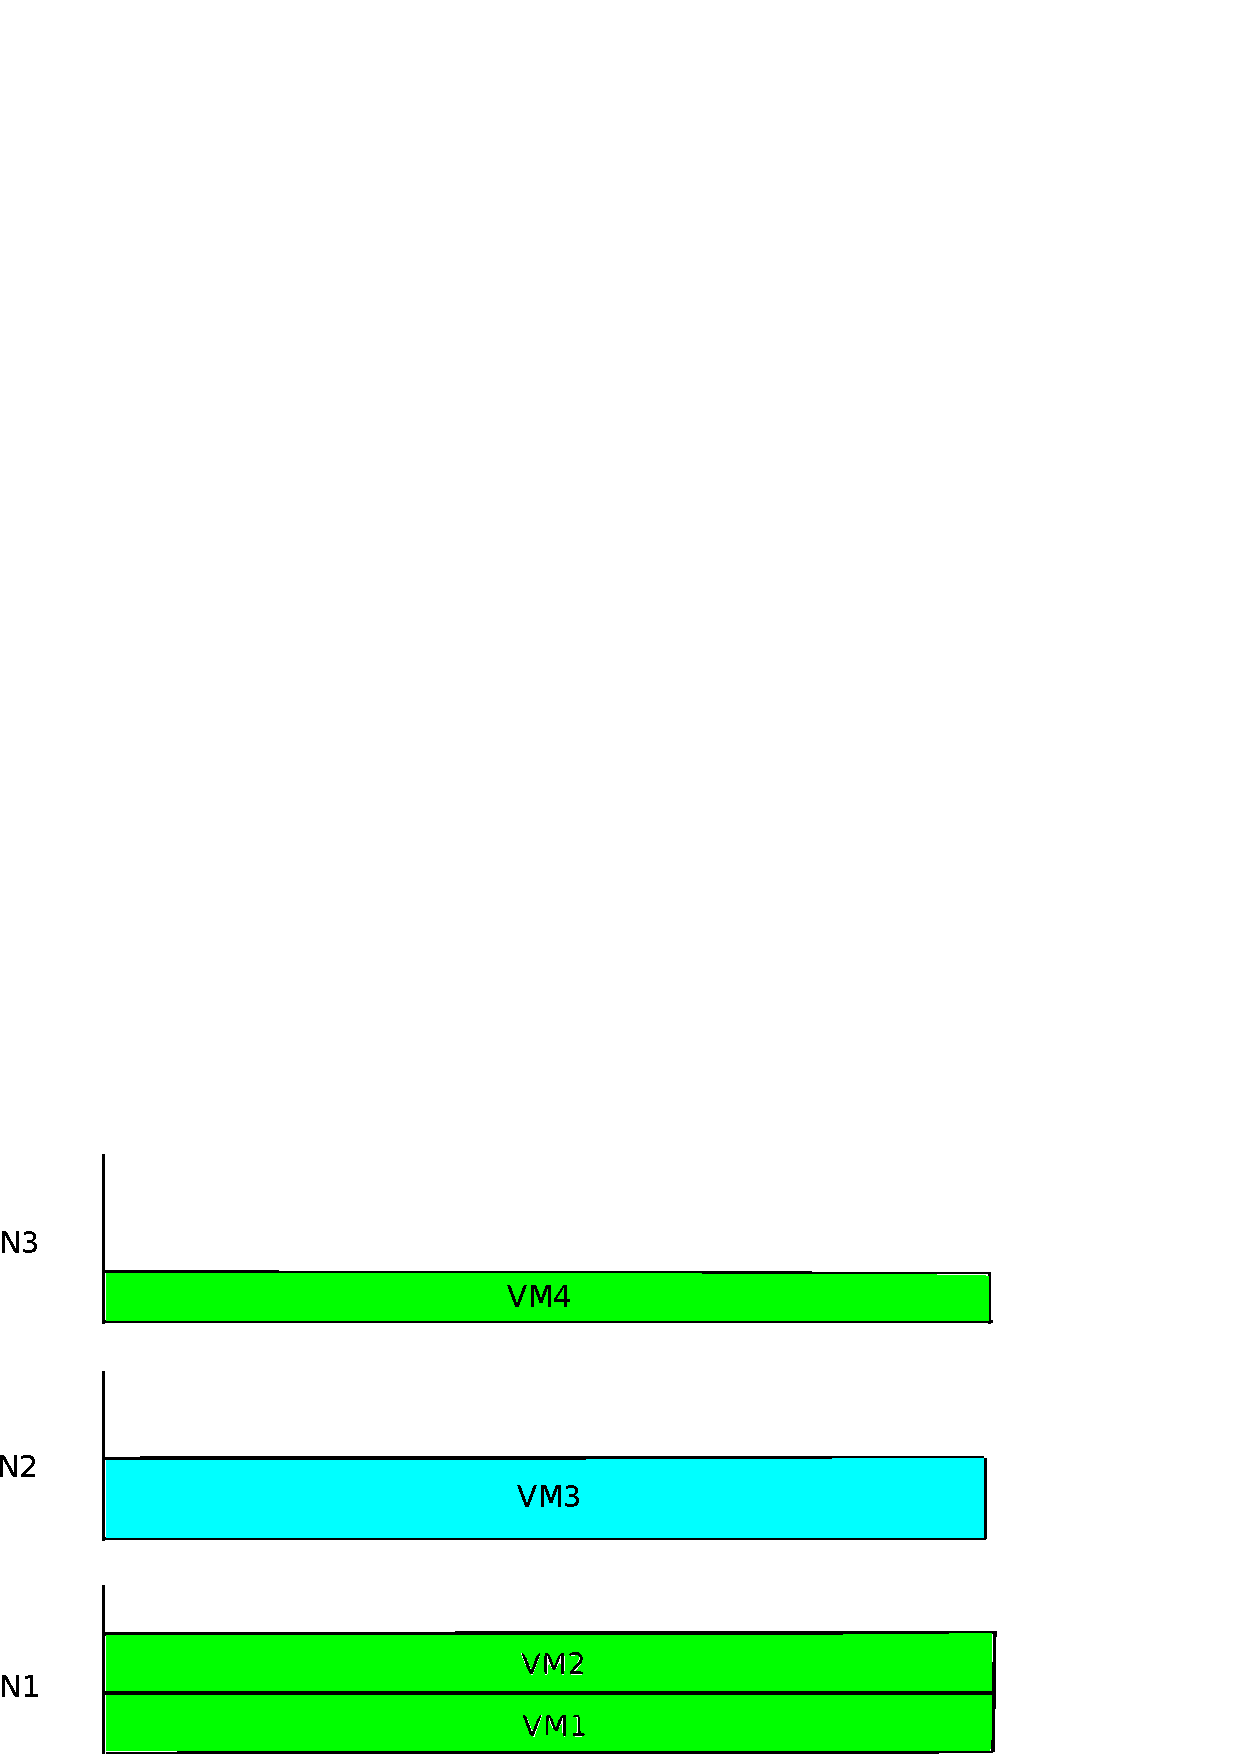
\includegraphics[scale=.25]{imgs/startreconf.png}
		\label{startreconf}
	}
	\subfigure[Après la reconfiguration] {
		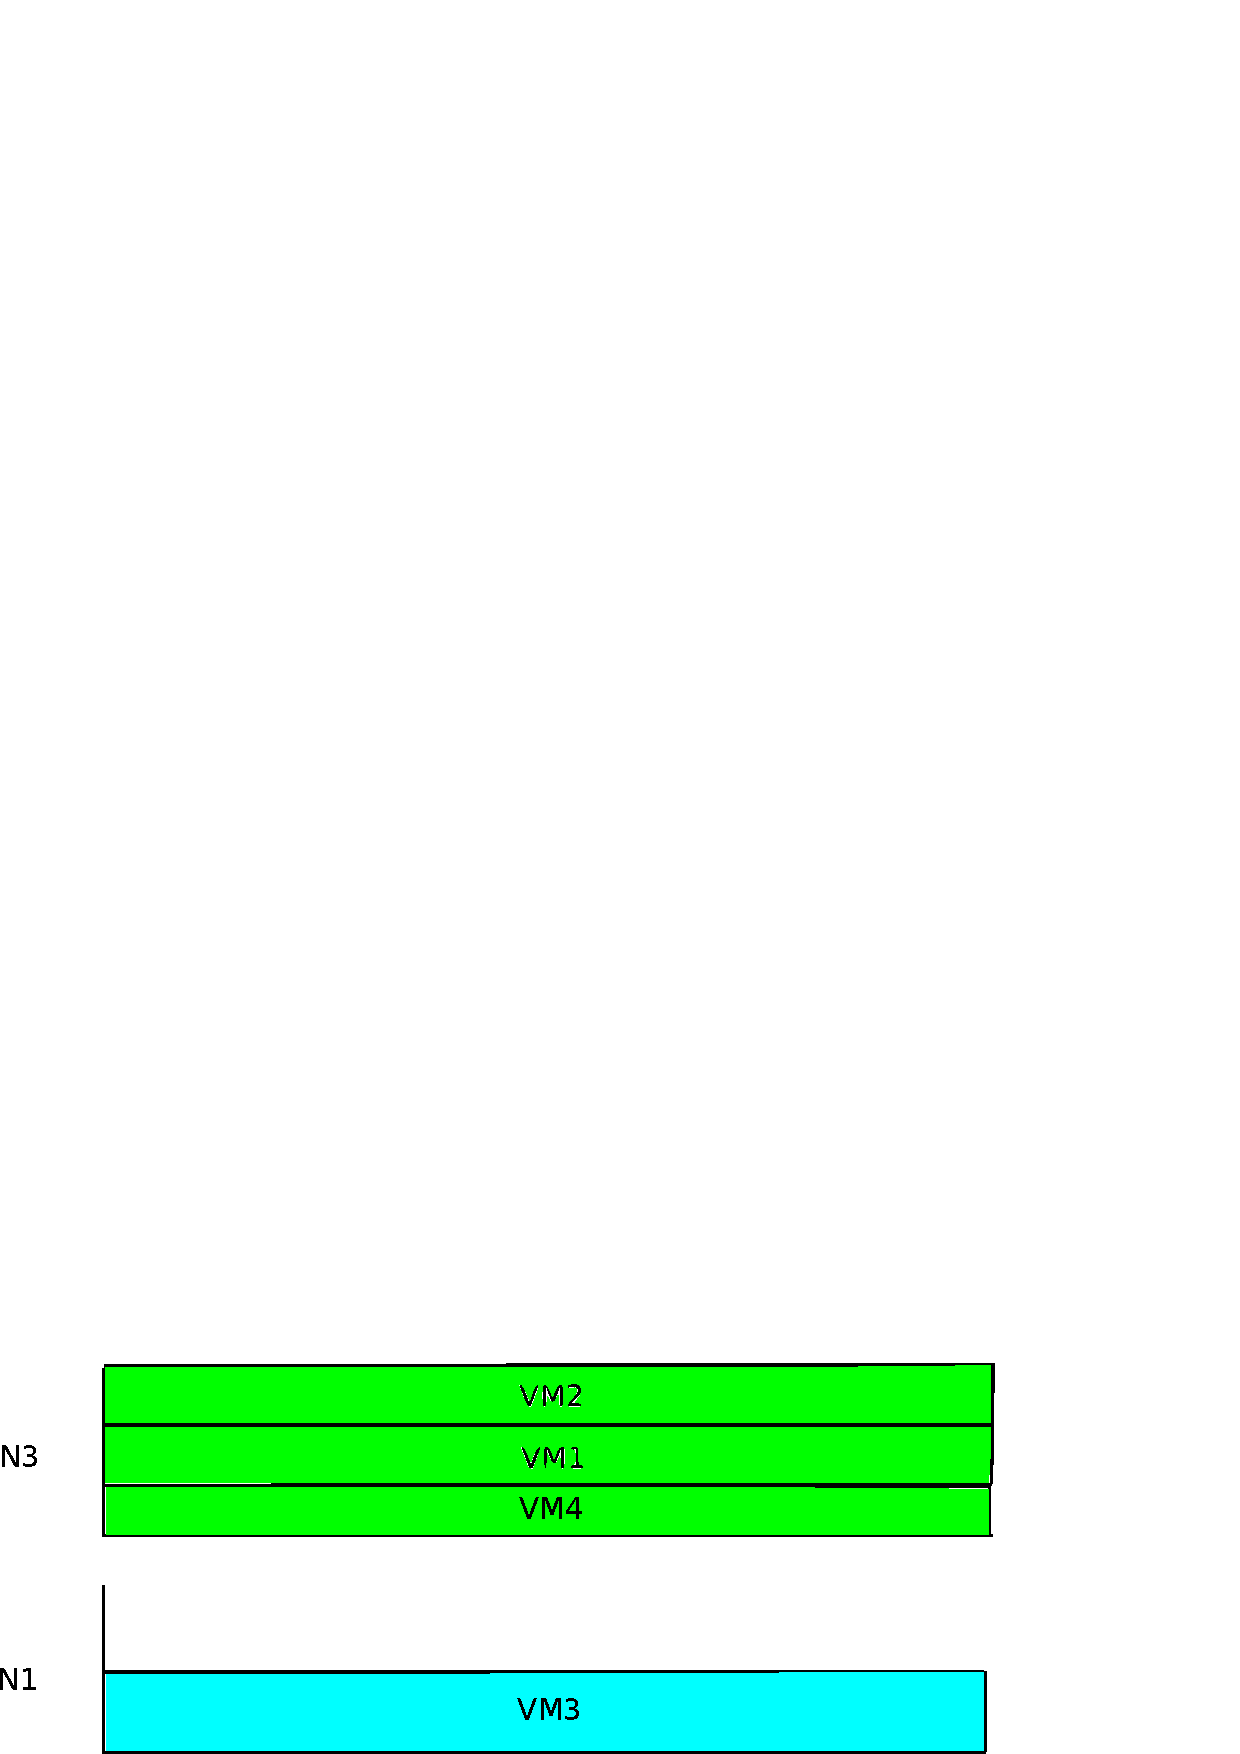
\includegraphics[scale=.25]{imgs/endreconf.png}
		\label{endreconf}
	}
	\caption{\label{usecase} Exemple de changement de système de
		virtualisation. En vert des VMs Xen, en cyan une VM VMWare}
\end{figure}

Sur le diagramme \ref{startreconf}, on souhait mettre le serveur physique
$N_2$ hors-ligne pour des questions de maintenance. On utilise pour cela
la contrainte \textit{offline($N_i$);}\footnote{\url{http://www-sop.inria.fr/members/Fabien.Hermenier/btrpcc/offline.html}}.

Comme aucun serveur VMWare n'est disponible, il est nécessaire de supprimer
un serveur Xen, capable d'accueillir $VM_3$, par exemple $N_1$. Les machines
virtuelles situées sur ce dernier, $VM_1$ et $VM_2$,  doivent dans un premier
temps être migrées sur un autre serveur.

Puis, $N_1$ doit s'éteindre et redémarrer en changeant son système
de virtualisation. Enfin, la $VM_3$ est déplacée sur $N_1$, et $N_2$ peut
être éteint, pour arriver dans l'état décrit par le diagramme \ref{endreconf}.

\subsection{Critère de succès}
Pour que le projet aboutisse, il est nécessaire d'établir un
formalisme mathématique correct pour représenter les différents
types de VMs supportés par les machines physiques.

\section{État de l'art}
\subsection{Description générale}
tralala
\subsection{Formalisation du problème}
On commence par définir le vocabulaire:
\begin{description}
	\item[Type] entier $t$ associé à chaque système de virtualisation;
	\item[VM] machine virtuelle, notée $v \in \mathcal V$, à laquelle
		est associée un type fixe $T(v)$ et une place $P(v)$;
	\item[Nœud] serveur physique, noté $n \in \mathcal N$,doté d'un
		type courant $T(n)$ et d'un ensemble de types possibles
		$\mathcal{T}_n$;
\end{description}

% On note $N_n$ le nombre de nœud; $N_v$ le nombre de VMs (c'est-à-dire
% respectivement les cardinaux de $\mathcal{N}$ et de $\mathcal{V}$).

La fonction $T$ associe à une VM ou un Nœud son type; la fonction $P$
associe à une VM un nœud.

Le placement est alors satisfait ssi chaque VM est bien placée sur
un nœud de même type, ie.:
\[
	(\forall v \in \mathcal V), (\exists n \in \mathcal N), P(v) = n
		\Rightarrow T(n) = T(v)	
\]

L'un des cas possible pour satisfaire cette condition et de changer le
type courant d'une machine virtuelle. Une action de déploiement doit
alors être mise en place.

La modélisation d'actions de reconfiguration est définie dans ~\cite{herm2012}.
Elles sont réalisées à l'aide de \textit{slices}, qui correspondent à
une durée finie pendant un processus de reconfiguration, durant laquelle
des ressources sont utilisées.
On distingue plusieurs types de slices:
\begin{description}
	\item[consuming slice], $c \in \mathcal C$, où les ressources sont
		utilisées au début de la reconfiguration;
	\item[demanding slice], $d \in \mathcal D$, où les ressources sont
		utilisées à la fin de la reconfiguration;
	\item[middle slice], $m \in \mathcal M$, où les ressources sont utilisées
		entre le début et la fin du processus (XXX ambigüe, notation).
\end{description}

L'opération de déploiement peut s'exprimer en fonction de ces slices:
\begin{enumerate}
	\item l'état initial (c-slice) lors de la reconfiguration contient les
		VMs de l'ancien type devant être déplacées sur un autre serveur ;
	\item l'état intermédiaire (m-slice) représente le changement de type,
		c'est-à-dire le changement de système de virtualisation. Il
		peut être vu comme consommant toutes les ressources disponibles
		sur le nœud;
	\item l'état final (d-slice) où les VMs du nouveau type sont migrées sur
		le nœud.
\end{enumerate}

\section{Méthodologie et planification}
\subsection{Stratégie générale}
bis repetita: trouver un bon formalisme; définir et implémenter
\subsection{Découpage en lots}
bis repetita: trouver un bon formalisme; définir et implémenter
\subsection{Plannification}
gantt
\subsection{Livrables associés au projet}
\begin{table}
\centering
\begin{tabular}{c|c|c|c|c}
	Id & Titre du livrable & Lot(s) & Nature & Date \\
	\hline
	\hline
	$D_0$ & Cahier des charges & $1$ & Document & $S_4$ \\
	\hline
	$D_1$ & Gestion du typage et du déploiement & $1$ & Document & $?$ \\
	\hline
	$D_2$ & Ensemble de contraintes & $1$ & Document et Logiciel & $?$ \\
	\hline
	$D_3$ & Rapport de management & $1$ & Document & $S_{20}$ \\
	\hline
	$D_4$ & Diaporama de présentation finale & $1$ & Document & $S_{20}$ \\
\end{tabular}
\end{table}

\subsection{Jalons}
\begin{table}
\centering
\begin{tabular}{c|c|c|c|c}
	Id & Jalon de fin de phase & Lot(s) & Date & Vérification \\
	\hline
	\hline
	$J_0$ & planification & $1$ & $S_4$ & $D_0$ \\
	\hline
	$J_1$ & formalisation & $1$ & $S_n$ & $D_1$ partiel \\
	\hline
	$J_2$ & implémentation & $1$ & $S_{n+k}$ & $D_2$, $D_1$ partiel \\
	\hline
	$J_3$ & projet & $1$ & $S_{20}$ & $D_1$, $D_2$, $D_3$ et $D_4$ \\
\end{tabular}
\end{table}

\section{Description de la mise en œuvre du projet}
\subsection{Interdépendance des lots et tâches}
bis repetita: trouver un bon formalisme; définir et implémenter
\subsection{Description des lots}
bis repetita: trouver un bon formalisme; définir et implémenter
\subsection{Résumé de l'effort}
\subsection{Gestion du risque}

\section{Participants}
\subsection{Mathieu Bivert - CSSR}
Étudiant à Polytech'Nice Sophia, spécialisé en Cryptographie, Systèmes
Sécurité et Réseaux.

\subsection{Fabien Hermenier - OASIS/INRIA}
\textbf{Fabien Hermenier} a recu un doctorat en $2009$ à l'université
de Nantes. Depuis $2011$, il enseigne en tant que professeur adjoint
à l'université de Nice Sophia-Antipolis. Son travail de recherche
s'articule autour des plateformes d'hébergement, de la virtualisation,
du calcul autonome et de la gestion des ressources. Depuis $2006$, il
travaille sur des algorithmes de placement de machines virtuelles pour
faire face à l'augmentation des SLA dans les plateformes d'hébergements.

\newpage
\selectlanguage{francais}
\bibliographystyle{alpha}
\bibliography{docs}

\end{document}

